\documentclass[manuscript,screen,review]{acmart}

\usepackage{graphicx}
\usepackage{longtable}
\usepackage{tikz}

\AtBeginDocument{
    \providecommand\BibTeX{{
        Bib\TeX}}}
\setcopyright{acmlicensed}
\copyrightyear{2024}
\acmYear{}
\acmDOI{}
\acmConference[]{}{,}{,}
\acmISBN{}

\begin{document}
\title{Guia teórico STEM Maker: Promovendo o Pensamento Computacional com Sensores e Microcontroladores para Engajar Estudantes em STEM}
\author{Douglas Aquino Teixeira Mendes}
\authornote{}
\email{douglasaquino4@gmail.com}
\orcid{0009-0009-7402-966X}
\affiliation{
  \institution{Universidade Federal de Lavras}
  \city{Lavras}
  \state{Minas Gerais}
  \country{Brasil}
}

\author{André de Lima Salgado}
\affiliation{%
  \institution{Universidade Federal de Lavras}
  \city{Lavras}
  \country{Brasil}}
\email{andrelima.salgado@gmail.com}

\author{Tales Heimfarth}
\affiliation{%
  \institution{Universidade Federal de Lavras}
  \city{Lavras}
  \country{Brasil}}
\email{tales@ufla.br}

\begin{abstract}
    Este estudo explora métodos para melhorar o ensino STEM através da análise automatizada de vídeos do YouTube. Utilizando técnicas de clusterização, foram identificados padrões de engajamento, transcrições e descrições visuais (captions) em vídeos educacionais. A metodologia incluiu a coleta de dados, processamento de áudio e texto, processamento de imagem e análise de engajamento. Os resultados destacam a importância de temas específicos e estilos de apresentação na retenção e interação do público. Além disso, o estudo apresenta uma explicação detalhada do algoritmo de Dijkstra, incluindo um exemplo prático de sua aplicação em um grafo de cidades conectadas por estradas. As conclusões fornecem recomendações baseadas em evidências para otimizar a produção de conteúdo educacional em plataformas de vídeo.

\end{abstract}

\keywords{STEM, STEM Maker, Sensores, Microcontroladores, Guia, Evasão}

\maketitle

\newpage 
\section{Introduction}

% \textbf{Contexto: } 
A dificuldade em conectar o pensamento computacional (PC) com as disciplinas STEM (Ciência, Tecnologia, Engenharia e Matemática) pode gerar desmotivação e dificuldades de aprendizagem, culminando na evasão. A falta de uma definição clara de como o PC se aplica em áreas específicas de STEM pode fazer com que os alunos não compreendam a relevância do PC para seus estudos \cite{Integrating}. Esse desafio é ainda mais evidente quando consideramos a necessidade de adaptar o ensino de PC para diferentes níveis de ensino, utilizando plataformas e linguagens de programação adequadas à faixa etária e aos objetivos de aprendizagem \cite{Analysis, Integrating}. A falta de confiança e autoeficácia também podem contribuir para a evasão, especialmente entre mulheres, que, apesar de demonstrarem competência em PC, muitas vezes, possuem menor confiança em suas habilidades \cite{Integrating}. A evasão pode ser exacerbada por experiências de aprendizagem desestimulantes e pela falta de acesso a recursos e oportunidades. \citet{Integrating,Assessing,Analysis,Measurement} enfatizam a importância de utilizar métodos de ensino inovadores e envolventes, como a metodologia STEM Maker, que incentiva a aprendizagem ativa e baseada em projetos. 

% \textbf{Revisão da literatura: } 
Atividades práticas, resolução de problemas e colaboração podem tornar o aprendizado mais significativo e eficaz \cite{Integrating,Assessing,Measurement,Preparing}, despertando o interesse dos alunos e combatendo a desmotivação. É crucial, também, garantir o acesso equitativo a recursos como computadores, softwares e oportunidades extracurriculares, especialmente para alunos de baixa renda ou de áreas rurais \cite{Preparing}.
É importante lembrar que a evasão é um problema complexo, influenciado por uma série de fatores que vão além do escopo apresentado. Para aprofundar a análise, seria necessário recorrer a estudos e pesquisas adicionais que explorem outras causas da evasão em STEM, como falta de apoio social, dificuldades financeiras, currículos desatualizados, estereótipos de gênero e raça, entre outros. 

O PC tem ganhado crescente atenção na educação STEM, sendo reconhecido como uma habilidade fundamental para o século XXI \cite{Assessing,Integrating}. No entanto, a definição e a aplicação do PC em contextos educacionais ainda geram debate \cite{Assessing,Integrating}.\citet{Integrating} demonstra que o PC pode ser compreendido de duas formas principais: uma definição genérica, que o define como um conjunto de habilidades para a resolução de problemas; e outra específica, que o adapta a diferentes disciplinas, como as áreas STEM. As definições genéricas de PC geralmente o descrevem como um processo que envolve a abstração, a decomposição, a generalização e o desenvolvimento de algoritmos para solucionar problemas \cite{Assessing,Integrating}. Um exemplo dessa abordagem é a definição da International Society for Technology in Education (ISTE) e da Computer Science Teachers Association (CSTA), que detalham as habilidades e disposições relacionadas ao PC na educação K-12 \cite{Integrating}. Já as definições específicas buscam integrar o PC aos conteúdos e práticas de cada disciplina, reconhecendo que a computação desempenha um papel fundamental nas áreas STEM modernas \cite{Integrating}.

Uma das abordagens que tem se destacado nesse contexto é a metodologia STEM Maker, que surge como uma abordagem promissora para integrar o PC em contextos STEM de forma prática e envolvente. O STEM Maker combina a cultura "maker" - que valoriza a experimentação e a construção de projetos - com os princípios da educação STEM, proporcionando aos alunos a oportunidade de aplicar o PC na criação de soluções para problemas reais \cite{Measurement}. \citet{Measurement} mostra que o STEM Maker pode ser utilizado em diferentes níveis de ensino, adaptando as ferramentas e as atividades à faixa etária dos alunos.

A relevância do PC e do STEM Maker reside na sua capacidade de preparar os estudantes para os desafios do século XXI. Em um mundo cada vez mais digital e tecnológico, a capacidade de solucionar problemas, pensar de forma crítica e criativa e trabalhar colaborativamente torna-se essencial \cite{Assessing}. O PC, por meio de atividades como programação, robótica e design de jogos, desenvolve essas habilidades e prepara os alunos para carreiras em áreas STEM e para a vida em sociedade \cite{Measurement,Integrating}.

% \textbf{Lacuna: } 
Um dos principais desafios na integração do pensamento computacional (PC) e do STEM Maker na educação é a falta de consenso sobre a definição do PC em contextos específicos de STEM. Isso pode gerar dificuldades para os educadores na hora de planejar as aulas e avaliar a aprendizagem dos alunos \cite{Assessing,Integrating}. Outro desafio é a necessidade de garantir o acesso equitativo a recursos e oportunidades de aprendizagem, especialmente para alunos de baixa renda ou de áreas rurais \cite{Assessing}. Em resumo, o PC e o STEM Maker são abordagens relevantes para a educação contemporânea, pois preparam os alunos para um mundo cada vez mais tecnológico e complexo. No entanto, para que essas abordagens sejam efetivas, é necessário superar os desafios de definição, avaliação e acesso, garantindo que todos os alunos tenham a oportunidade de desenvolver habilidades essenciais para o século XXI.

% \textbf{Propósito: } 
A integração de sensores inerciais e microcontroladores na educação STEM oferece uma conexão prática entre teoria e aplicação, permitindo que conceitos abstratos, como aceleração e forças, sejam explorados por meio de experimentos interativos \cite{Measurement}. Essas ferramentas promovem maior engajamento ao proporcionar resultados em tempo real, característica essencial do ambiente STEM Maker, onde o aprendizado ocorre de forma prática e exploratória. Além de estimular o desenvolvimento de habilidades críticas do século XXI, como pensamento computacional e solução de problemas, esses dispositivos preparam os estudantes para demandas tecnológicas do mercado de trabalho. Projetos envolvendo sensores também permitem a integração de temas de saúde e bem-estar, como o monitoramento biomecânico, conectando a ciência ao cotidiano de forma significativa. Com um custo relativamente acessível e suporte de comunidades ativas, microcontroladores como Arduino tornam-se viáveis para implementação em projetos escolares, inspirando estudantes a se tornarem criadores e inovadores, capazes de resolver problemas reais e contribuir para a sociedade. 

Este guia tem como objetivo fornecer uma base teórica para a criação de materiais educacionais voltados para a promoção do pensamento computacional (PC) e o engajamento de estudantes em disciplinas STEM (Ciência, Tecnologia, Engenharia e Matemática). A proposta centra-se no uso de abordagens STEM Maker integrando sensores inerciais e microcontroladores, demonstrando como essas tecnologias podem ser utilizadas em projetos práticos e interativos. O objetivo final é fornecer um guia estruturado que inspire educadores a adotar práticas STEM Maker, com potencial para reduzir a evasão em disciplinas STEM ao estimular um aprendizado ativo, colaborativo e significativo. O guia busca:

\begin{itemize}
    \item Apresentar atividades e projetos teóricos que combinem conceitos STEM com a aplicação de sensores e microcontroladores, sem a necessidade de testes empíricos diretos.
    \item  Incorporar exemplos de vídeos, tutoriais e ferramentas amplamente disponíveis, validados pela comunidade, para facilitar a implementação de projetos.
    \item  Propor atividades que conectem conceitos acadêmicos a temas cotidianos, como saúde e bem-estar, aumentando a relevância e a atratividade das disciplinas STEM.
    \item  Demonstrar como essas tecnologias, devido ao seu custo acessível e ampla disponibilidade, podem ser usadas em diferentes contextos educacionais e níveis de ensino.
\end{itemize}

\textbf{Método}: Este estudo é de natureza exploratória e utilizou uma análise temática de vídeos publicamente disponíveis em mídias sociais, com foco no ensino de algoritmos e estruturas de dados. A seleção dos vídeos foi realizada com base em um protocolo PICO, em que a população foi definida como educadores e estudantes de STEM, a intervenção como sensores, microcontroladores e atividades práticas, e o desfecho como métricas de engajamento, incluindo visualizações e "curtidas". Os resultados das buscas foram ordenados pela quantidade de visualizações, utilizada como principal métrica de sucesso nas redes sociais. A análise temática envolveu a codificação inicial de características empregadas no ensino nos vídeos selecionados, repetindo-se o processo até a saturação teórica, quando nenhum novo tema foi identificado. Os temas codificados, links dos vídeos e métricas de engajamento foram registrados em um dataset, que posteriormente foi analisado por meio de técnicas de agrupamento para identificar padrões de nível mais alto. O objetivo foi estruturar um guia de boas práticas didáticas no ensino de algoritmos e estruturas de dados, baseado nos temas identificados.

%\newpage
\section{Metodologia}

Para a realização desta pesquisa sobre como melhorar o ensino STEM, foi desenvolvida uma abordagem baseada em análise automatizada de vídeos do YouTube. O processo metodológico seguiu as seguintes etapas:

\begin{itemize}
    \item \textbf{Materiais:} 
    Para este estudo, foram utilizados vídeos publicamente disponíveis na plataforma de mídia social YouTube, abordando o ensino de algoritmos e estruturas de dados. As ferramentas empregadas incluíram um protocolo PICO para a construção da string de busca e planilhas eletrônicas para registro de dados (como links, visualizações, métricas de engajamento e anotações de padrões nos temas extraídos).

    \item \textbf{Procedimento:} 
    A pesquisa foi conduzida iniciando pela Definição do Protocolo PICO, para definir a população, a intervenção e o desfecho. Assim, com o tema principal e seus sinônimos definidos, foi possível criar uma string de busca. O tema e os sinônimos definidos podem ser observados na Tabela \ref{tab:PICO}. 

    \begin{table}[ht]
    \centering
    \begin{tabular}{|p{3cm}|p{4cm}|p{7cm}|}
    \hline
    \textbf{Ponto de Vista} & \textbf{Tema Principal} & \textbf{Sinônimos/Termos Relacionados} \\ \hline
    População (P)           & Educadores e Estudantes de STEM &  Professores, Instrução,  Alunos, Aprendizes, Computação, Science, Technology, Programação, Engineering, Mathematics, Algorithms \\ \hline
    Intervenção (I)         & STEM Maker, Microcontroladores e Sensores & Atividades práticas, faça você mesmo, Movimento, Sensores IMU\\ \hline
    Comparação (C)          & Aula expositiva tradicional & - \\ \hline
    Desfecho (O)            & Métricas de engajamento & curtidas, comentários \\ \hline
    \end{tabular}
    \caption{Estrutura PICO com temas principais e sinônimos.}
    \label{tab:PICO}
    \end{table}

    \item \textbf{Coleta de Dados:} 
    Foram desenvolvidos scripts em Python para realizar pesquisas automáticas no YouTube. As strings de busca foram elaboradas utilizando a metodologia PICO, garantindo maior precisão na identificação de conteúdos relevantes. Os vídeos resultantes das buscas foram baixados, juntamente com as métricas de engajamento, incluindo número de likes e visualizações.

    \item \textbf{Processamento de Áudio e Texto:} 
    O áudio dos vídeos foi transcrito para texto. As transcrições foram normalizadas para remoção de ruídos textuais e palavras irrelevantes. O texto resultante foi vetorizado e submetido a um processo de clusterização para identificar padrões temáticos entre os vídeos analisados.

    \item \textbf{Processamento de Imagem e Geração de Descrições:} 
    Foram extraídas capturas de tela (screenshots) a cada 10 segundos de cada vídeo. Utilizou-se o modelo BlipProcessor para gerar descrições automáticas (captions) para cada frame. O processo gerou um total de 9.819 captions, com um tempo de processamento estimado em 5 horas. As captions foram normalizadas, vetorizadas e submetidas a um processo de clusterização para identificação de padrões visuais e semânticos.

    \item \textbf{Análise de Engajamento:} 
    O engajamento dos vídeos foi calculado com base na relação entre likes e views. Os valores de engajamento foram vetorizados e clusterizados para identificar padrões entre os conteúdos analisados.

    \item \textbf{Clusterização em Segunda Ordem:} 
    Os vídeos foram agrupados em clusters de segunda ordem, levando em consideração os clusters temáticos previamente identificados. Essa etapa permitiu encontrar vídeos que abordam o mesmo assunto de maneira similar e possuem boa avaliação por parte dos usuários.

    \item \textbf{Definição do Número de Clusters:} 
    Em todas as etapas de clusterização, foi utilizado o método do cotovelo (elbow method) para definir o número ideal de clusters.
\end{itemize}

As etapas descritas acima permitiram a criação de uma estrutura analítica para compreender padrões na disseminação de conteúdos STEM no YouTube, possibilitando futuras recomendações baseadas em evidências para o aprimoramento do ensino nessa área.

\section{Resultados}

\subsection{Método do Cotovelo}

O método do cotovelo é uma técnica utilizada para determinar o número ótimo de clusters em um conjunto de dados. Ele consiste em calcular a soma dos erros quadráticos dentro dos clusters (within-cluster sum of squares - WCSS) para diferentes valores de k (número de clusters) e \textit{plotar} um gráfico com esses valores. O ponto onde há uma inflexão acentuada no gráfico — formando um "cotovelo" — indica o número ideal de clusters, pois após esse ponto, o ganho na redução da variabilidade dentro dos clusters se torna marginal.

\subsection{Gráficos Gerados}

A seguir, são apresentados os gráficos gerados para cada uma das etapas da análise:

\begin{itemize}
    \item \textbf{Engajamento dos vídeos:} O gráfico do cotovelo mostrou um ponto de inflexão claro, como é possível visualizar na Figura \ref{fig:elbow_engajamento}, permitindo a definição justificada do número de clusters.
    
    \begin{figure}[ht]
        \centering
        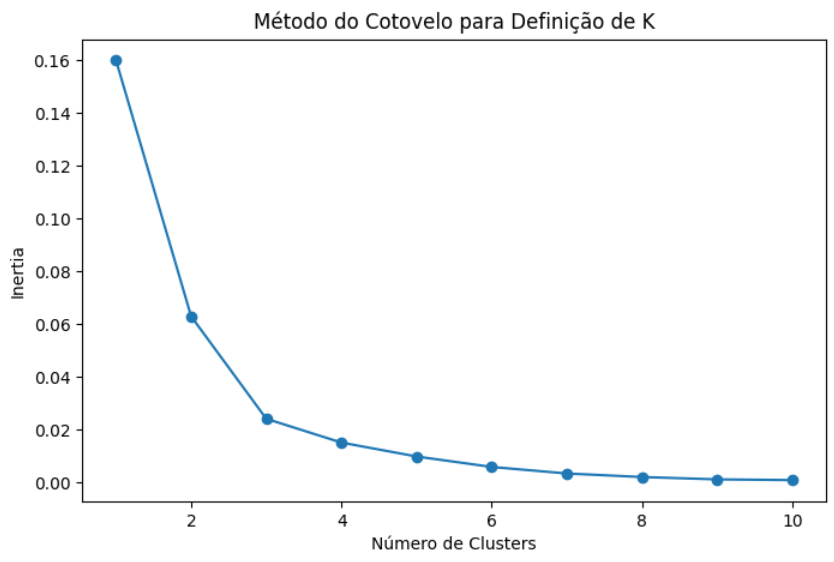
\includegraphics[width=0.7\columnwidth]{../../Classifica_videos/Images/cotovelo_engage.png}
        \caption{Gráfico do método do cotovelo para o engajamento dos vídeos.}
        \label{fig:elbow_engajamento}
    \end{figure}

    \item \textbf{Captações automáticas (captions):} O gráfico gerado apresentou uma reta descendente, ilustrado na Figura \ref{fig:elbow_captions}, indicando que a variabilidade não apresentou uma quebra nítida para definir um número exato de clusters.
    
    \item \textbf{Transcrições:} Assim como no caso das captions, a curva do cotovelo ilustrado na Figura \ref{fig:elbow_transcripts} mostrou uma tendência descendente contínua, sem um ponto de inflexão bem definido. Isso pode indicar que a variabilidade dos dados não permite uma separação clara em clusters distintos.
    
    \begin{figure}
        \centering
        \begin{minipage}{0.45\textwidth}
            \centering
            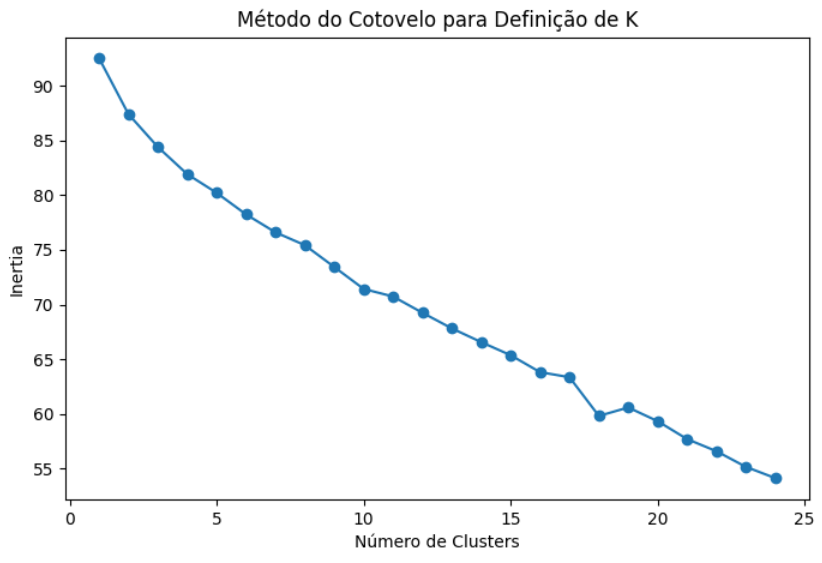
\includegraphics[width=\linewidth]{../../Classifica_videos/Images/cotovelo_captions.png}
            \caption{Gráfico do método do cotovelo para as captions.}
            \label{fig:elbow_captions}
        \end{minipage}
        \hfill
        \begin{minipage}{0.45\textwidth}
            \centering
            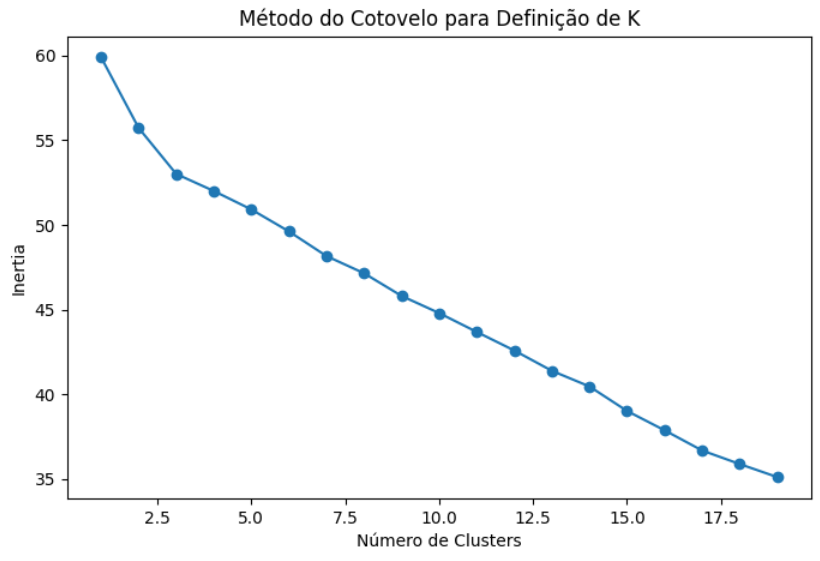
\includegraphics[width=\linewidth]{../../Classifica_videos/Images/cotovelo_transcripts.png}
            \caption{Gráfico do método do cotovelo para as transcrições.}
            \label{fig:elbow_transcripts}
        \end{minipage}
        \caption{Graficos que geraram uma reta descendente}
    \end{figure}

    \item \textbf{Clusterização global:} O gráfico indicou um ponto de cotovelo bem definido, como é possível identificar na Figura \ref{fig:elbow_global}, justificando a escolha do número ótimo de clusters para a organização dos vídeos analisados.
    
    \begin{figure}
        \centering
        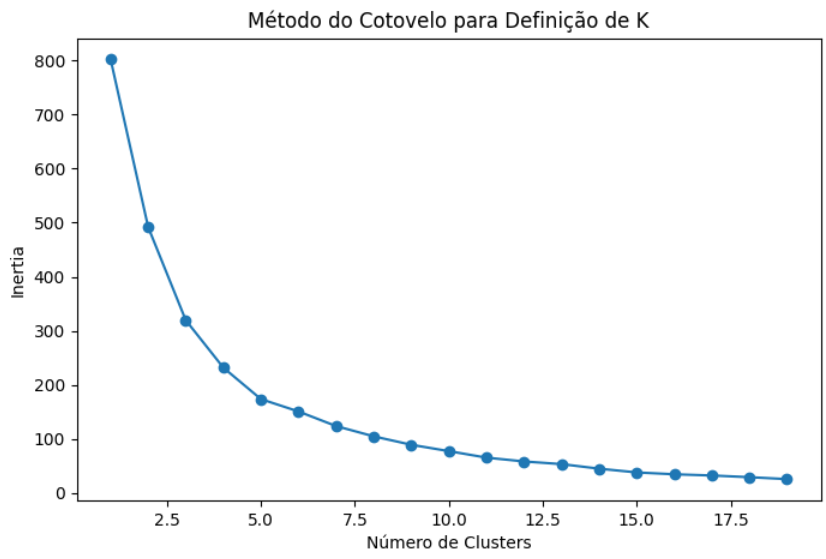
\includegraphics[width=0.7\columnwidth]{../../Classifica_videos/Images/cotovelo_global.png}
        \caption{Gráfico do método do cotovelo para a clusterização global.}
        \label{fig:elbow_global}
    \end{figure}
\end{itemize}


\subsection{Clusterização dos Dados}

A clusterização foi aplicada a diferentes aspectos dos vídeos analisados, conforme descrito abaixo:

\begin{itemize}
    \item \textbf{Clusterização do Engajamento:} 
    O engajamento dos vídeos foi agrupado em 5 clusters, utilizando a métrica de likes/views como critério principal. Essa abordagem permitiu segmentar vídeos com alto, médio e baixo engajamento, como pode ser observado na Figura \ref{fig:cluster_engage}, possibilitando a identificação de padrões de popularidade e relevância.

    \begin{figure}[h]
        \centering
        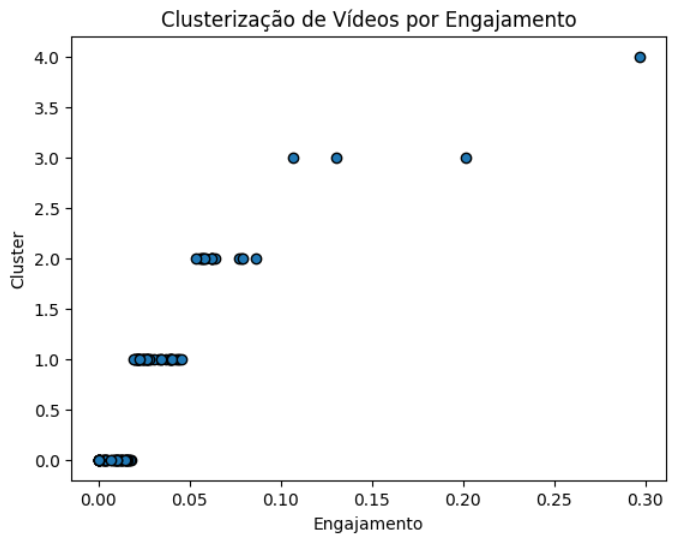
\includegraphics[width=0.7\columnwidth]{../../Classifica_videos/Images/cluster_engage.png}
        \caption{Clusterização do engajamento dos vídeos.}
        \label{fig:cluster_engage}
    \end{figure}

    \item \textbf{Clusterização das Transcrições:} 
    O conteúdo textual dos vídeos foi agrupado em 5 clusters. Esse processo permitiu identificar padrões temáticos recorrentes nos vídeos analisados.

    \item \textbf{Clusterização das Captions:} 
    As captions geradas automaticamente foram também agrupadas em 5 clusters. Essa análise revelou padrões visuais e semânticos nos vídeos, auxiliando na categorização dos conteúdos.

    \item \textbf{Clusterização Global (Segunda Ordem):} 
    A clusterização global foi realizada utilizando 9 clusters. Essa abordagem permitiu agrupar vídeos que tratam de um mesmo assunto de forma similar e possuem avaliações positivas.
\end{itemize}

\begin{longtable}{|c|c|c|c|c|}
    \hline
ID & cluster\_engage & cluster\_transcript & cluster\_caption & cluster\_global \\
\hline
\endfirsthead
\hline
ID & cluster\_engage & cluster\_transcript & cluster\_caption & cluster\_global \\
\hline
\endhead
\hline
    7Usk\_Gcn\_hc & 2 & 2 & C & 0 \\
PTelAW-QYVI & 1 & 2 & C & 0 \\
Soj850lcZiA & 2 & 2 & C & 0 \\
1ibpxkWlcoE & 2 & 2 & B & 0 \\
CSVzWR98Tk8 & 2 & 0 & E & 0 \\
go-xrFCqP9g & 2 & 2 & B & 0 \\
TNMWuO-viDc & 2 & 2 & B & 0 \\
63LbwNScJAM & 1 & 2 & C & 0 \\
Ca340RM9zhA & 2 & 4 & C & 0 \\
VsHECCRhjXk & 2 & 2 & A & 0 \\
AVlggsXkiLc & 2 & 2 & B & 0 \\
rrLwckDaYsc & 2 & 0 & E & 0 \\
N8XdchwemrU & 0 & 2 & A & 1 \\
fiO27fz3DJI & 0 & 2 & A & 1 \\
ffxpAExL8Ok & 0 & 2 & A & 1 \\
URFUBzk0ff8 & 1 & 2 & E & 1 \\
KVLTxKyxioA & 1 & 2 & B & 1 \\
8h-B0v6qa0A & 1 & 1 & D & 1 \\
IkxkU2xquKY & 1 & 2 & E & 1 \\
z8T29GYPlVM & 1 & -1 & A & 1 \\
rebIOhS7L\_M & 1 & 2 & E & 1 \\
rAOKLGKWa5I & 1 & 2 & A & 1 \\
kEYlGbgg9Kw & 1 & 1 & A & 1 \\
85WsCSmW3Xc & 1 & 2 & A & 1 \\
ECzzX0PfIeE & 1 & 2 & D & 1 \\
posTc56basM & 3 & 4 & A & 1 \\
IItwxAzoMXs & 1 & 0 & E & 1 \\
ltL3q16mPvk & 1 & 2 & E & 1 \\
lgD\_G0\_5EYE & 1 & 4 & E & 1 \\
Te1ov1q5P1I & 1 & 4 & A & 1 \\
o-2s9sM8YS4 & 0 & 2 & A & 1 \\
gxiUxd9Zkbg & 1 & 4 & D & 1 \\
9IVxOTuRVBk & 2 & 4 & E & 2 \\
6XuPwdESzqc & 2 & 3 & B & 2 \\
6Th-RGQShjc & 2 & 4 & A & 2 \\
zO5lxz3Tmxo & 2 & 4 & B & 2 \\
tmYUZSytIdE & 2 & 4 & B & 2 \\
Ciiyz68E3a0 & 2 & 4 & B & 2 \\
mg7VAT0bEcg & 1 & 4 & B & 2 \\
htmJbUtFmKE & 3 & 4 & B & 2 \\
Zuigm5JqxQs & 3 & 1 & B & 2 \\
lpYPEUJObQ0 & 0 & 2 & E & 3 \\
0wyyX1FspRE & 0 & 2 & E & 3 \\
yoOQgGkYGZ0 & 0 & 2 & B & 3 \\
9JY2vuxdWnU & 0 & 2 & B & 3 \\
nhuxzE016oU & 0 & 2 & B & 3 \\
3ziIdlgJQTk & 0 & 2 & B & 3 \\
FOjRjrlPg3o & 0 & 2 & B & 3 \\
0GTpRnUBveA & 0 & 2 & B & 3 \\
Ia1QXHPfKJw & 0 & 2 & B & 3 \\
dyRqPLKCvO4 & 4 & 2 & B & 3 \\
7fCC4xob94A & 0 & -1 & C & 4 \\
lkFejnE\_6Mo & 0 & -1 & C & 4 \\
tRbpSljw5-s & 0 & 3 & C & 4 \\
FEtprl6I9\_w & 0 & 3 & C & 4 \\
kEFwaP4\_6FM & 0 & -1 & C & 4 \\
TCttcJjnxfs & 0 & -1 & A & 4 \\
oyRjS\_6hGtk & 0 & -1 & E & 4 \\
7Q22PHY6nP8 & 0 & -1 & C & 4 \\
HFTRoBMGGOI & 0 & -1 & C & 4 \\
ksG87OUZOkA & 0 & -1 & C & 4 \\
FFBSI9VGphA & 0 & -1 & C & 4 \\
jvZBRHiLKiE & 0 & -1 & E & 4 \\
7UKiv4KsZDg & 0 & -1 & C & 4 \\
MRDBYz3PCXQ & 0 & -1 & B & 5 \\
QUUKCluhPT0 & 0 & -1 & B & 5 \\
87wbUWUF68Y & 0 & -1 & B & 5 \\
pvGVFzlikYc & 0 & -1 & B & 5 \\
JN2aSu\_NXLo & 0 & -1 & B & 5 \\
0XtoXITfDy8 & 1 & -1 & C & 6 \\
5Auq\_8z\_qSg & 1 & -1 & C & 6 \\
6FliHIDP5fo & 1 & -1 & D & 6 \\
6yJJfFjb2z0 & 1 & -1 & C & 6 \\
4bdXOms1BeU & 1 & -1 & C & 6 \\
bf9BYmYPqkE & 1 & -1 & D & 6 \\
lmv4YmB-q5A & 1 & -1 & C & 6 \\
Pbzb\_n9XNJ0 & 1 & -1 & E & 6 \\
7oc0yCeOLGE & 1 & -1 & E & 6 \\
giaCldbGKAQ & 1 & -1 & C & 6 \\
f3CK3mE\_r9c & 1 & 4 & C & 6 \\
BFgqhoX5BE4 & 1 & -1 & C & 6 \\
o7DMHJKhpws & 1 & -1 & C & 6 \\
BqbLCoPGxNg & 1 & -1 & E & 6 \\
AvKY1yCwB8o & 1 & -1 & C & 6 \\
yZmKNx0G5eE & 1 & -1 & C & 6 \\
CtvO3yZZmpA & 1 & -1 & C & 6 \\
Q9r4Kvr8Qsg & 1 & -1 & C & 6 \\
WUCBeeATyMU & 1 & -1 & C & 6 \\
Mc2z8Y0jAZs & 1 & -1 & E & 6 \\
V3NJdxTRRts & 1 & -1 & C & 6 \\
wy2iLgERLkE & 0 & 2 & D & 7 \\
SBh6dJMM6AI & 0 & 1 & D & 7 \\
eGdxXGJglLQ & 0 & 1 & D & 7 \\
Y9lGSRcIQ68 & 0 & 2 & D & 7 \\
14XvT5iEfns & 0 & 2 & D & 7 \\
tELhGLWkuZY & 0 & 2 & D & 7 \\
VHiacccJw7g & 0 & 2 & C & 8 \\
T7YEmRTa5MQ & 0 & 2 & C & 8 \\
JOfCZohKHrw & 0 & 2 & C & 8 \\
G0OyNjTZs84 & 0 & 2 & C & 8 \\
24YsiQewxeQ & 0 & 2 & C & 8 \\
\hline
\caption{Mapa de calor com os clusters de dados}
\end{longtable}

\newpage
\section{Discussões}
A análise dos clusters apresentados sugere que, teoricamente, o método utilizado para identificar os vídeos mais relevantes pode ser eficaz para a escolha de conteúdos de maior engajamento. Ao observar os gráficos que comparam o "Cluster Final" e o "Cluster de Engajamento", na Figura \ref{fig:heatmap}, é possível fazer algumas observações que auxiliam na interpretação dos dados.

\begin{figure}[ht]
    \centering
    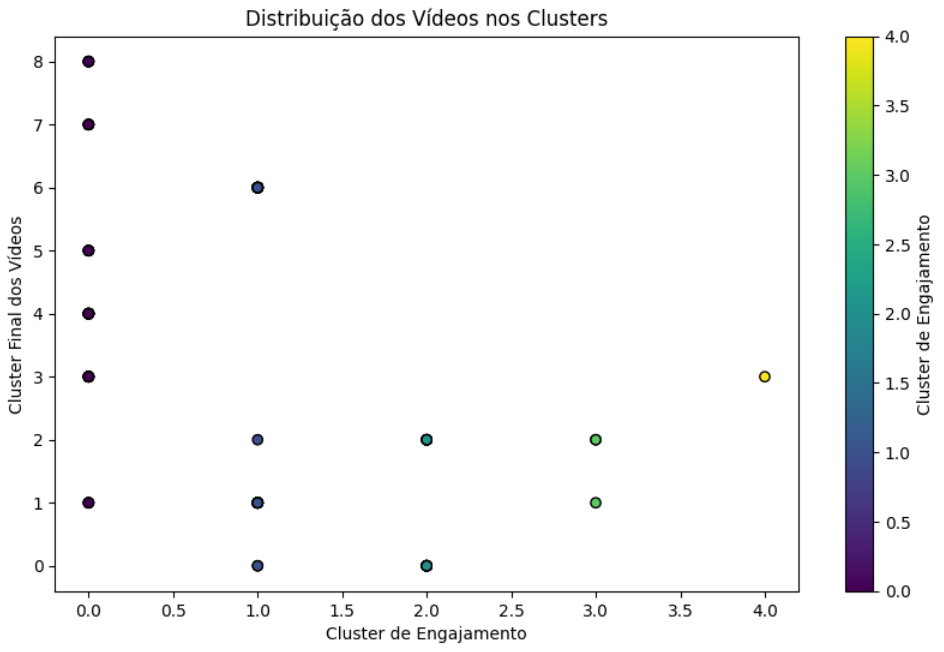
\includegraphics[width=0.7\columnwidth]{../../Classifica_videos/Images/finalXengage.png}
    \caption{Mapa de calor com os clusters finais e de engajamento.}
    \label{fig:heatmap}
\end{figure}

Primeiramente, o \textit{cluster final} 3, apesar de incluir o vídeo com o melhor engajamento, apresenta uma grande quantidade de vídeos com o menor índice de engajamento. Este fenômeno pode indicar que canais menos populares ou em fase inicial estão se inspirando em vídeos que já possuem um engajamento consolidado, mas não obtêm o mesmo sucesso. Essa discrepância sugere que o sucesso de um vídeo não depende apenas de sua qualidade ou popularidade, mas também de outros fatores, como o perfil do canal ou da audiência.

Por outro lado, os \textit{clusters} 1, 2 e 0 revelam, teoricamente, os vídeos com melhor desempenho em termos de engajamento, com uma distribuição mais equilibrada. Esses clusters apresentam uma média de engajamento satisfatória, sugerindo que esses vídeos podem ser considerados como boas fontes de inspiração para outros canais. O sucesso nesses clusters pode ser atribuído a um equilíbrio adequado entre conteúdo relevante e a capacidade de atrair a audiência.

Em contraste, os \textit{clusters} 8, 7, 6, 5 e 4 apresentam os vídeos com os piores níveis de engajamento. Essa observação pode indicar que os vídeos desses clusters falham em atrair o público de maneira eficaz, e, portanto, sugerem que uma análise mais detalhada do conteúdo desses vídeos poderia revelar práticas que devem ser evitadas. Durante as aulas, seria relevante investigar as características desses vídeos e identificar quais aspectos podem ser melhorados, como a qualidade do conteúdo, a interação com o público ou até mesmo fatores técnicos relacionados à apresentação. Os gráficos e análises aqui discutidos fornecem uma base teórica para entender o comportamento dos vídeos em relação ao engajamento, e podem orientar futuras estratégias de criação de conteúdo.

Ao analisar o gráfico de Captions em Cluster Final X Engajamento, ilustrado na Figura \ref{fig:captionsFinal}, é possível identificar padrões que reforçam algumas das observações anteriores e trazem novos insights sobre a relação entre o conteúdo abordado e o nível de engajamento do público.

\begin{figure}
    \centering
    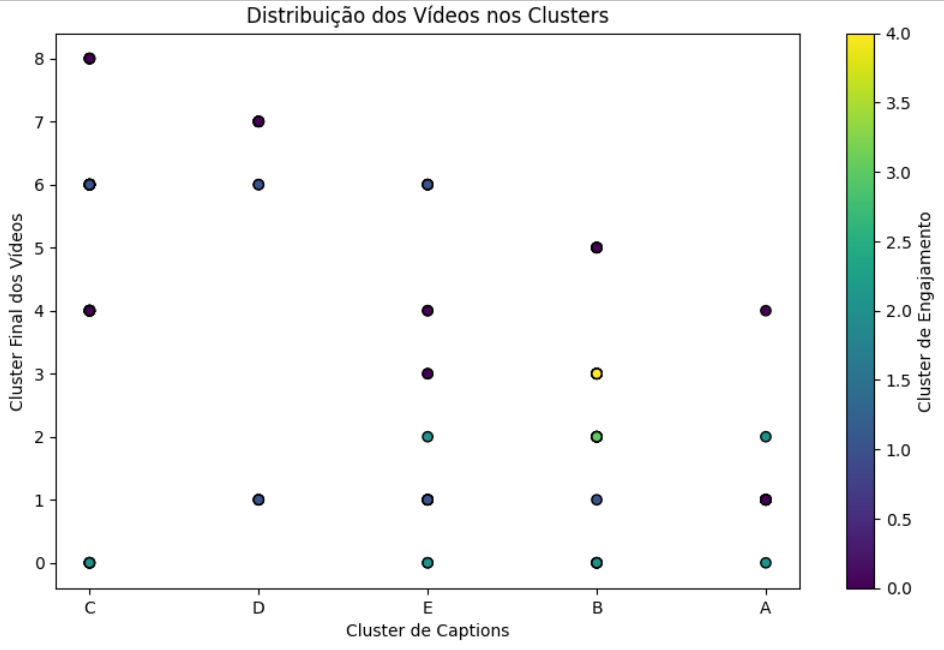
\includegraphics[width=0.7\columnwidth]{../../Classifica_videos/Images/finalXengageXcaption.png}
    \caption{Mapa de calor com os clusters finais, de engajamento e de captions.}
    \label{fig:captionsFinal}
\end{figure}

O \textit{Cluster B} se destaca como a forma de exibir o tema, mais bem avaliado, sugerindo que vídeos que abordam esse assunto exibindo de tal maneira, tendem a gerar maior interesse e envolvimento por parte dos espectadores. Além disso, os clusters 2 e 0 novamente aparecem como os que apresentam os melhores resultados de engajamento, o que indica que os vídeos classificados nesses grupos conseguem explorar os temas de forma eficaz, mantendo um nível médio-alto de interação com o público. Esse resultado sugere que a forma do Cluster B, como os vídeos abordam o tema, está melhor representada no Cluster Final 2, evidenciando um padrão de comunicação mais eficaz.

Por outro lado, os clusters 8, 7, 5 e 4, assim como observado na análise anterior, continuam apresentando baixos índices de engajamento. Esse comportamento reforça a hipótese de que os vídeos agrupados nesses clusters podem conter características que prejudicam a retenção da audiência, sendo que pela forma de apresentação dos clusters C e D, aparenta ser a pior maneira de exibir o conteúdo.

O Cluster 1 apresenta um desempenho mediano em termos de engajamento, porém, com uma maior diversidade de métodos. Esse aspecto pode indicar que a variação temática pode impactar os níveis de engajamento, possivelmente tornando o desempenho menos previsível ou dificultando a formação de uma audiência fiel.

Essas observações reforçam a importância de compreender como determinados temas e estilos de apresentação influenciam o sucesso das apresentações de um conteúdo. A análise detalhada dos clusters pode ajudar a identificar as melhores práticas e estratégias para otimizar a produção de conteúdo, garantindo maior engajamento e relevância dentro da plataforma.

Por fim, ao analisar o gráfico de Transcrições no Cluster Final, ilustrado na Figura \ref{fig:transcriptFinal}, podemos observar a relação entre o conteúdo falado nos vídeos e o nível de engajamento obtido. A transcrição representa o que foi dito no áudio dos vídeos, permitindo identificar quais temas e abordagens influenciam diretamente na interação do público.

\begin{figure}
    \centering
    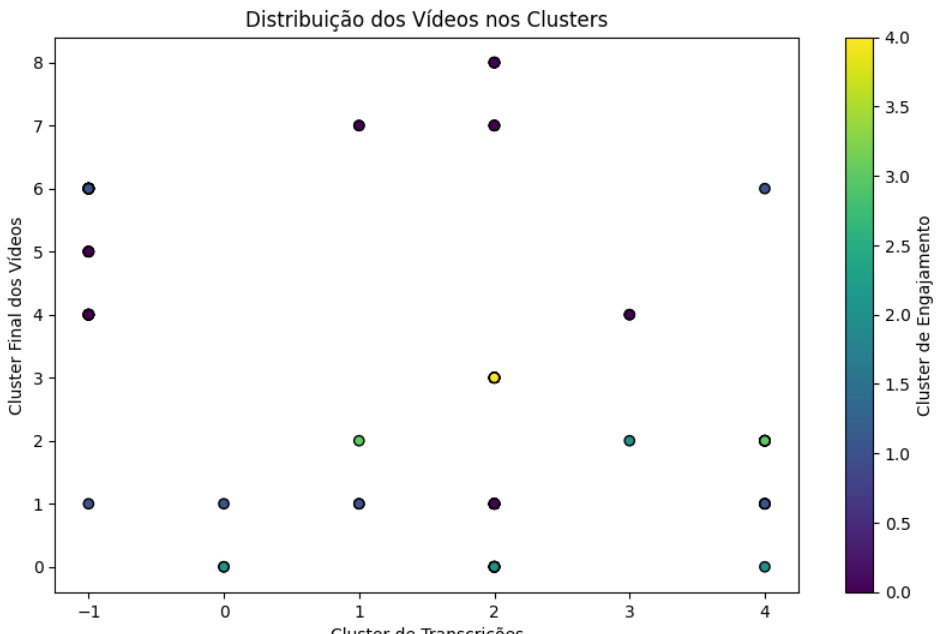
\includegraphics[width=0.7\columnwidth]{../../Classifica_videos/Images/finalXengageXtranscript.png}
    \caption{Mapa de calor com os clusters finais, de engajamento e de transcrições.}
    \label{fig:transcriptFinal}
\end{figure}

O Assunto 2 apresenta a maior variação de engajamento, sugerindo que ele pode ser abordado de formas distintas nos vídeos, gerando tanto altos quanto baixos níveis de interação. No entanto, essa variação indica que o Cluster Final 3 consegue apresentar esse assunto da maneira mais eficaz, resultando em um engajamento mais expressivo em alguns vídeos.

Os Assuntos 0 e 4 demonstram uma média de engajamento satisfatória, indicando que esses temas, quando bem desenvolvidos, contribuem para manter a atenção do público e gerar interações. Por outro lado, os clusters 8, 7, 6, 5 e 4 continuam apresentando um desempenho abaixo da média, reforçando o padrão observado nas análises anteriores. Isso sugere que vídeos classificados nesses grupos podem possuir características que impactam negativamente a retenção e o envolvimento dos espectadores.

Um ponto relevante é a presença do Assunto -1, que representa vídeos onde não há falas, apenas elementos visuais sendo apresentados. Os dados indicam que esses vídeos possuem engajamentos consistentemente baixos, sugerindo que a simples exibição do conteúdo, sem explicação ou contextualização verbal, não é suficiente para capturar o interesse da audiência. Esse resultado reforça a importância da comunicação falada na construção de um vídeo mais envolvente e eficaz.

Com base nessas observações, podemos concluir que a forma como os temas são abordados desempenha um papel fundamental no engajamento do público. A análise das transcrições permite identificar quais estilos de apresentação são mais eficientes e pode servir como referência para otimizar a criação de conteúdos futuros, visando melhorar a interação e retenção da audiência.

\section{Explicação do Algoritmo de Dijkstra}

O algoritmo de Dijkstra é um método para encontrar o caminho mais curto entre um nó de origem e os demais nós em um grafo ponderado, desde que os pesos das arestas sejam não negativos. Ele é amplamente utilizado em problemas de roteamento, redes e sistemas de navegação.

\subsection{Passos do Algoritmo}

\begin{itemize}
    \item \textbf{Inicialização:}
    \begin{itemize}
        \item Definir um nó inicial e atribuir a ele uma distância de 0.
        \item Todos os outros nós recebem uma distância inicial infinita ($\infty$), pois ainda não foram alcançados.
        \item Criar uma estrutura para armazenar os nós visitados.
    \end{itemize}

    \item \textbf{Processamento dos Nós:}
    \begin{itemize}
        \item Selecionar o nó não visitado com a menor distância conhecida (inicialmente, o nó inicial).
        \item Atualizar as distâncias de seus vizinhos diretos. Se a distância encontrada for menor do que a anteriormente registrada, substituí-la.
        \item Marcar o nó atual como visitado, pois sua menor distância já foi determinada.
    \end{itemize}

    \item \textbf{Repetição do Processo:}
    \begin{itemize}
        \item Continuar o processo para o próximo nó não visitado com a menor distância.
        \item Repetir até que todos os nós tenham sido processados ou até que o nó destino tenha sido alcançado.
    \end{itemize}

    \item \textbf{Construção do Caminho:}
    \begin{itemize}
        \item Ao final, a estrutura de dados utilizada permite reconstruir o caminho mais curto do nó inicial até qualquer outro nó alcançável.
    \end{itemize}
\end{itemize}

\subsection{Exemplo Prático}

Considere um grafo representado por cidades conectadas por estradas, onde os pesos representam as distâncias entre elas. Se quisermos encontrar o caminho mais curto entre a cidade $A$ e a cidade $D$, o algoritmo seguirá os passos mencionados, sempre escolhendo a menor distância acumulada e evitando recalcular caminhos já determinados.

\begin{figure}[h]
    \centering
    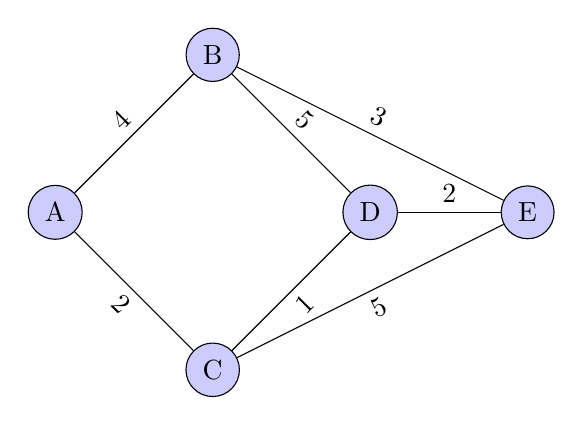
\begin{tikzpicture}
        % Nodes
        \node (A) at (0,0) [circle, draw, fill=blue!20] {A};
        \node (B) at (2,2) [circle, draw, fill=blue!20] {B};
        \node (C) at (2,-2) [circle, draw, fill=blue!20] {C};
        \node (D) at (4,0) [circle, draw, fill=blue!20] {D};
        \node (E) at (6,0) [circle, draw, fill=blue!20] {E};

        % Edges
        \draw (A) -- (B) node[midway, above, sloped] {4};
        \draw (A) -- (C) node[midway, below, sloped] {2};
        \draw (B) -- (D) node[midway, above, sloped] {5};
        \draw (C) -- (D) node[midway, below, sloped] {1};
        \draw (C) -- (E) node[midway, below, sloped] {5};
        \draw (D) -- (E) node[midway, above, sloped] {2};
        \draw (B) -- (E) node[midway, above, sloped] {3};
    \end{tikzpicture}
    \caption{Exemplo de grafo com cidades e distâncias.}
    \label{fig:grafo_exemplo}
\end{figure}

\begin{itemize}
    \item \textbf{Passo 1: Inicialização}
    \begin{itemize}
        \item Definir a cidade $A$ como o nó inicial e atribuir a ela uma distância de 0.
        \item Todas as outras cidades ($B$, $C$, $D$, $E$) recebem uma distância inicial infinita ($\infty$).
        \item Criar uma estrutura para armazenar as cidades visitadas (inicialmente vazia).
    \end{itemize}

    \item \textbf{Passo 2: Processamento dos Nós}
    \begin{itemize}
        \item Selecionar a cidade $A$ (nó inicial) com a menor distância conhecida (0).
        \item Atualizar as distâncias de seus vizinhos diretos ($B$ e $C$):
        \begin{itemize}
            \item Distância para $B$: $0 + 4 = 4$
            \item Distância para $C$: $0 + 2 = 2$
        \end{itemize}
        \item Marcar a cidade $A$ como visitada.
    \end{itemize}

    \item \textbf{Passo 3: Repetição do Processo}
    \begin{itemize}
        \item Selecionar a cidade não visitada com a menor distância conhecida ($C$ com distância 2).
        \item Atualizar as distâncias de seus vizinhos diretos ($D$ e $E$):
        \begin{itemize}
            \item Distância para $D$: $2 + 1 = 3$
            \item Distância para $E$: $2 + 5 = 7$
        \end{itemize}
        \item Marcar a cidade $C$ como visitada.
        \item Selecionar a cidade não visitada com a menor distância conhecida ($D$ com distância 3).
        \item Atualizar as distâncias de seus vizinhos diretos ($E$):
        \begin{itemize}
            \item Distância para $E$: $3 + 2 = 5$ (menor que a distância anterior de 7)
        \end{itemize}
        \item Marcar a cidade $D$ como visitada.
        \item Selecionar a cidade não visitada com a menor distância conhecida ($B$ com distância 4).
        \item Atualizar as distâncias de seus vizinhos diretos ($E$):
        \begin{itemize}
            \item Distância para $E$: $4 + 3 = 7$ (não é menor que a distância anterior de 5)
        \end{itemize}
        \item Marcar a cidade $B$ como visitada.
        \item Selecionar a cidade não visitada com a menor distância conhecida ($E$ com distância 5).
        \item Marcar a cidade $E$ como visitada.
    \end{itemize}

    \item \textbf{Passo 4: Construção do Caminho}
    \begin{itemize}
        \item Ao final, a estrutura de dados utilizada permite reconstruir o caminho mais curto do nó inicial $A$ até qualquer outro nó alcançável.
        \item Caminho mais curto de $A$ a $D$: $A \rightarrow C \rightarrow D$ com distância total de 3.
    \end{itemize}
\end{itemize}

\begin{figure}[h]
    \centering
    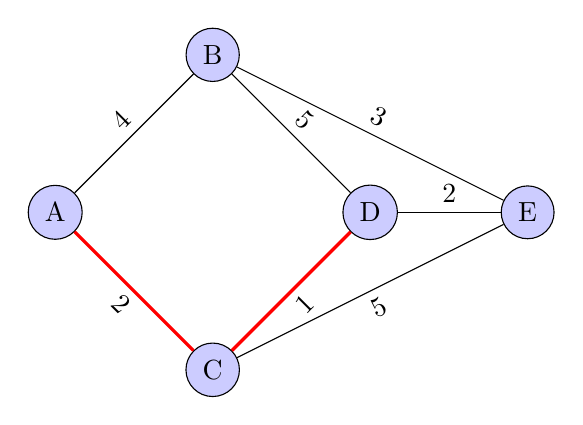
\begin{tikzpicture}
        % Nodes
        \node (A) at (0,0) [circle, draw, fill=blue!20] {A};
        \node (B) at (2,2) [circle, draw, fill=blue!20] {B};
        \node (C) at (2,-2) [circle, draw, fill=blue!20] {C};
        \node (D) at (4,0) [circle, draw, fill=blue!20] {D};
        \node (E) at (6,0) [circle, draw, fill=blue!20] {E};

        % Edges
        \draw (A) -- (B) node[midway, above, sloped] {4};
        \draw (A) -- (C) node[midway, below, sloped] {2};
        \draw (B) -- (D) node[midway, above, sloped] {5};
        \draw (C) -- (D) node[midway, below, sloped] {1};
        \draw (C) -- (E) node[midway, below, sloped] {5};
        \draw (D) -- (E) node[midway, above, sloped] {2};
        \draw (B) -- (E) node[midway, above, sloped] {3};

        % Highlighted path
        \draw[very thick, red] (A) -- (C);
        \draw[very thick, red] (C) -- (D);
    \end{tikzpicture}
    \caption{Exemplo de grafo com cidades e distâncias, destacando o caminho mais curto de A a D.}
    \label{fig:grafo_exemplo}
\end{figure}

\bibliographystyle{ACM-Reference-Format}
\bibliography{refs}

\end{document}

